\section{Results and Discussions}
\label{sec:results_and_discussions}

\vspace{-0.2cm}

\subsection{Timing}

\begin{wrapfigure}{R}{0.45\linewidth}
	\vspace{-2.7cm}
	\begin{center}
		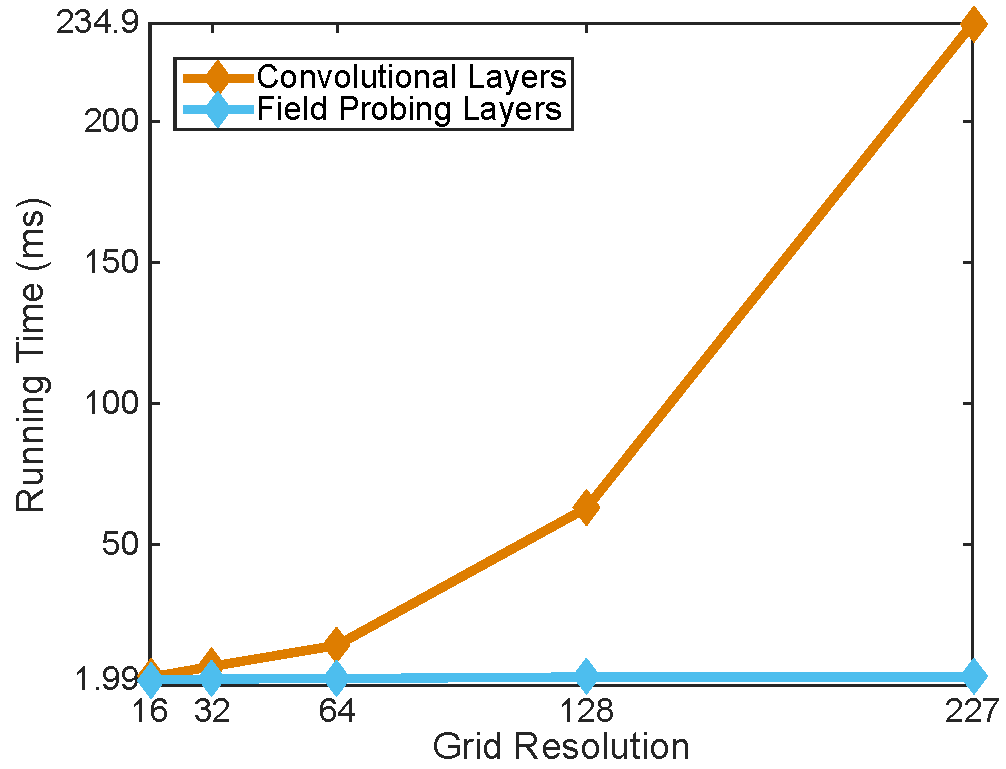
\includegraphics[width=1.0\linewidth]{figures/timing_v2}
	\end{center}
	\vspace{-0.4cm}
	\caption{Running time of convolutional layers (same settings as that in~\protect\cite{WU_CVPR15_3D}) and field probing layers ($C \times N \times T = 1024 \times 8 \times 4$) on Nvidia GTX TITAN with batch size $8$\protect\footnotemark.}
	\label{fig:timing}
	\vspace{-0.2cm}
\end{wrapfigure}
\footnotetext{The batch size is chosen to make sure the largest resolution data fits well in GPU memory.}

We implemented our field probing layers in Caffe~\cite{Jia_arXiv14_Caffe}. The Sensor layer is parallelized by assigning computation on each probing point to one GPU thread, and DotProduct layer by assigning computation on each probing filter to one GPU thread. Figure~\ref{fig:timing} shows a run time comparison between convonlutional layers and field probing layers on different input resolutions. The computation cost of our field probing layers is agnostic to input resolutions, the slight increase of the run time on higher resolution is due to GPU memory latency introduced by the larger 3D fields. Note that the convolutional layers in~\cite{Jia_arXiv14_Caffe} are based on highly optimized cuBlas library from NVIDIA, while our field probing layers are implemented with our naive parallelism, which is likely to be further improved.

\vspace{-0.2cm}
\subsection{Datasets and Evaluation Protocols}
We use ModelNet40~\cite{WU_CVPR15_3D} (12,311 models from 40 categories, training/testing split with 9,843/2,468 models\footnote{The split is provided on the authors' website. In their paper, a split composed of at most 80/20 training/testing models for each category was used, which is tiny for deep learning tasks and thus prone to overfitting. Therefore, we report and compare our performance on the whole ModelNet40 dataset.}) --- the standard benchmark for 3D object classification task, in our experiments. Models in this dataset are already aligned with a canonical orientation. For 3D object recognition scenarios in real world, the gravity direction can often be captured by the sensor, but the horizontal ``facing'' direction of the objects are unknown. We augment ModelNet40 data by randomly rotating the shapes horizontally. Note that this is done for both training and testing samples, thus in the testing phase, the orientation of the inputs are unknown. This allows us to assess how well the trained network perform on real world data.

\subsection{Performance of Field Probing Layers}

\begin{wraptable}{R}{0.5\linewidth}
%\begin{table}
	\vspace{-2.1cm}
	\begin{center}
		\scalebox{0.9}{
	\begin{tabular}{ | c | c | c | c | c | c |}
		\hline
		\multicolumn{3}{|c|}{1-FC} & \multicolumn{3}{c|}{4-FCs} \\
		\hline
		w/o FP & w/ FP & +NF & w/o FP & w/ FP & +NF \\
		\hline
		 79.1 & 85.0 & 86.0 & 86.6 & 87.5 & 88.4  \\
		\hline
	\end{tabular}
	}
	\end{center}
	\vspace{-0.2cm}
	\caption{Top-1 accuracy of FPNNs on 3D object classification task on $ModelNet40$ dataset.}
	\label{tab:performance_evaluation}
	\vspace{-0.2cm}
%\end{table}
\end{wraptable}

We train our FPNN $80,000$ iterations on $64 \times 64 \times 64$ distance field with batch size $1024$.\footnote{To save disk I/O footprint, a data augmentation is done on the fly. Each iteration, $256$ data samples are loaded, and augmented into $1024$ samples for a batch.}, with SGD solver, learning rate $0.01$, momentum $0.9$, and weight decay $0.0005$.

Trying to study the performance of our field probing layers separately, we build up an FPNN with only one fully connected layer that converts the output of field probing layers into the representation for softmax classification loss (1-FC setting). Batch normalization~\cite{ioffe2015batch} and rectified-linear unit~\cite{nair2010rectified} are used in-between our field probing layers and the fully connected layer for reducing internal covariate shift and introducing non-linearity. We train the network without/with updating the field probing layer parameters. We show their top-1 accuracy on 3D object classification task on $ModelNet40$ dataset with single testing view in Table~\ref{tab:performance_evaluation}. It is clear that our field probing layers learned to sense the input field more intelligently, with a $5.9\%$ performance gain from $79.1\%$ to $85.0\%$. Note that, what achieved by this simple network, $85.0\%$, is already better than the state-of-the-art 3DCNN before~\cite{qi2016volumetric} ($83.0\%$ in~\cite{WU_CVPR15_3D} and $83.8\%$ in~\cite{Maturana_IROS15_VoxNet}).

We also evaluate the performance of our field probing layers in the context of a deeper FPNN, where four fully connected layers\footnote{The first three of them output $1024$ dimensional feature vector.}, with in-between batch normalization, rectified-linear unit and Dropout~\cite{srivastava2014dropout} layers, are used (4-FCs setting). As shown in Table~\ref{tab:performance_evaluation}, the deeper FPNN performs better, while the gap between with and without field probing layers, $87.5\%-86.6\%=0.9\%$, is smaller than that in one fully connected FPNN setting. This is not surprising, as the additional fully connected layers, with many parameters introduced, have strong learning capability. The $0.9\%$ performance gap introduced by our field probing layers is a precious extra over a strong baseline.

It is important to note that in both settings (1-FC and 4-FCs), our FPNNs provides reasonable performance even without optimizing the field probing layers. This confirms that long range connections among the sensors are beneficial.

Furthermore, we evaluate our FPNNs with multiple input fields (+NF setting). We did not only employ distance fields, but also normal fields for our probing layers and found a consistent performance gain for both of the aforementioned FPNNs (see Table~\ref{tab:performance_evaluation}). Since normal fields are derived from distance fields, the same group of probing filters are used for both fields. Employing multiple fields in the field probing layers with different groups of filters potentially enables even higher performance.

\begin{wraptable}{R}{0.5\linewidth}
%\begin{table}
	\vspace{-0.9cm}
	\begin{center}
		\scalebox{0.75}{
	\begin{tabular}{ | c | c | c | c | c | c | c |}
		\hline
		FPNN Setting & $R$ & $R_{15}$ & $R_{15}+T_{0.1}+S$ & $R_{45}$ & $T_{0.2}$\\
		\hline
		1-FC & 85.0 & 82.4 & 76.2 & 74.1 & 72.2\\
		\hline
		4-FCs & 87.5 & 86.8 & 84.9 & 85.3 & 85.4 \\
		\hline
		\cite{WU_CVPR15_3D} & 84.7 & - & - & 83.0 & 84.8 \\
		\hline
	\end{tabular}
	}
	\end{center}
	\vspace{-0.3cm}
	\caption{Performance on different perturbations.}
	\label{tab:robustness}
	\vspace{-0.5cm}
%\end{table}
\end{wraptable}

\paragraph{Robustness Against Spatial Perturbations.} We evaluate our FPNNs on different levels of spatial perturbations, and summarize the results in Table~\ref{tab:robustness}, where $R$ indicates random horizontal rotation, $R_{15}$ indicates $R$ plus a small random rotation ($-15\degree$, $15\degree$) in the other two directions, $T_{0.1}$ indicates random translations within range ($-0.1$, $0.1$) of the object size in all directions, $S$ indicates random scaling within range ($0.9$, $1.1$) in all directions. $R_{45}$ and $T_{0.2}$ shares the same notations, but with even stronger rotation and translation, and are used in~\cite{qi2016volumetric} for evaluating the performance of~\cite{WU_CVPR15_3D}. Note that such perturbations are done on both training and testing samples. It is clear that our FPNNs are robust against spatial perturbations.

\begin{wraptable}{R}{0.5\linewidth}
%\begin{table}
	\vspace{-1.2cm}
	\begin{center}
		\scalebox{0.9}{
	\begin{tabular}{ | c | c | c | c | c |}
		\hline
		FPNN Setting & $0.2-0.8$ & $0.2-0.4$ & $0.1-0.2$ \\
		\hline
		1-FC & 85.0 & 84.1 & 82.8 \\
		\hline
		4-FCs & 87.5 & 86.8 & 86.9 \\
		\hline
	\end{tabular}
	}
	\end{center}
	\vspace{-0.3cm}
	\caption{Performance with different filter spans.}
	\label{tab:long_range}
	\vspace{-0.4cm}
%\end{table}
\end{wraptable}
\paragraph{Advantage of Long Range Connections.}
We evaluate our FPNNs with different range parameters $[l_{low}, l_{high}]$ used in initializing the probing filters, and summarize the results in Table~\ref{tab:long_range}. Note that since the output dimensionality of our field probing layers is low enough to be directly feed into fully connected layers, distant sensor information is directly coupled by them. This is a desirable property, however, it poses the difficulty to study the advantage of field probing layers in coupling long range information separately. Table~\ref{tab:long_range} shows that even if the following fully connected layer has the capability to couple distance information, the long range connections introduced in our field probing layers are beneficial.

\begin{wraptable}{R}{0.5\linewidth}
%\begin{table}
	\vspace{-0.8cm}
	\begin{center}
		\scalebox{0.75}{
	\begin{tabular}{ | c | c | c | c | c |}
		\hline
		FPNN Setting & \small{$16 \times 16 \times 16$} & \small{$32 \times 32 \times 32$} & \small{$64 \times 64 \times 64$} \\
		\hline
		1-FC & 84.2 & 84.5 & 85.0 \\
		\hline
		4-FCs & 87.3 & 87.3 & 87.5 \\
		\hline
	\end{tabular}
	}
	\end{center}
	\vspace{-0.3cm}
	\caption{Performance on different field resolutions.}
	\label{tab:field_resolution}
	\vspace{-0.3cm}
%\end{table}
\end{wraptable}
\paragraph{Performance on Different Field Resolutions.}
We evaluate our FPNNs on different input field resolutions, and summarize the results in Table~\ref{tab:field_resolution}. Higher resolution input fields can represent input data more accurately, and Table~\ref{tab:field_resolution} shows that our FPNN can take advantage of the more accurate representations. Since the computation cost of our field probing layers is agnostic to the resolution of the data representation, higher resolution input fields are preferred for better performance, while coupling with efficient data structures reduces the I/O footprint.

\paragraph{``Sharpness'' of Gaussian Layer.} The $\sigma$ hyper-parameter in Gaussian layer controls how ``sharp'' is the transform. We select its value empirically in our experiments, and the best performance is given when we use $\sigma \approx 10\%$ of the object size. Smaller $\sigma$ slightly hurts the performance ($\approx 1\%$), but has the potential of reducing I/O footprint.

\begin{wrapfigure}{R}{0.6\linewidth}
	\vspace{-1.5cm}
	\begin{center}
		\includegraphics[width=1.0\linewidth]{figures/embedding_space_lower}
	\end{center}
	\vspace{-0.5cm}
	\caption{t-SNE visualization of FPNN features.}
	\label{fig:embedding_space}
	\vspace{-0.4cm}
\end{wrapfigure}

\paragraph{FPNN Features and Visual Similarity.} Figure~\ref{fig:embedding_space} shows a visualization of the features extracted by the FPNN trained for a classification task. Our FPNN is capable of capturing 3D geometric structures such that it allows to map 3D models that belong to the same categories (indicated by colors) to similar regions in the feature space. More specifically, our FPNN maps 3D models into points in a high dimensional feature space, where the distances between the points measure the similarity between their corresponding 3D models. As can be seen from Figure~\ref{fig:embedding_space} (better viewed in zoomin mode),  the FPNN feature distances between 3D models represent their shape similarities, thus FPNN features can support shape exploration and retrieval tasks.

\subsection{Generalizability of FPNN Features}
\begin{wraptable}{R}{0.5\linewidth}
\vspace{-2.1cm}
\begin{center}
	\scalebox{0.78}{
\begin{tabular}{ | c | c | c | c |}
  \hline
    \multirow{2}{*}{Testing Dataset} & \multirow{2}{*}{FP+FC} & \multirow{2}{*}{FC Only} & FP+FC on Source \\
     &  &  & FC Only on Target \\
	\hline
	${MN40}_1$ & 93.8 & 90.7 & 92.7 \\
	\hline
	${MN40}_2$ & 89.4 & 85.1 & 88.2 \\
	\hline
\end{tabular}
}
\end{center}
\vspace{-0.3cm}
\caption{Generalizability test of FPNN features.}
\label{tab:generality_test}
\vspace{-0.4cm}
\end{wraptable}
One superior characteristic of CNN features is that features from one task or dataset can be transferred to another task or dataset. We evaluate the generalizability of FPNN features by cross validation --- we train on one dataset and test on another. We first split ${ModelNet40}$ (lexicographically by the category names) into two parts ${MN40}_1$ and ${MN40}_2$, where each of them contains $20$ non-overlapping categories. Then we train two FPNNs in a 1-FC setting (updating both field probing layers and the only one fully connected layer) on these two datasets, achieving $93.8\%$ and $89.4\%$ accuracy, respectively (the second column in Table~\ref{tab:generality_test}).\footnote{The performance is higher than that on all the $40$ categories, since the classification task is simpler on less categories. The performance gap between ${MN40}_1$ and ${MN40}_2$ is presumably due to the fact that ${MN40}_1$ categories are easier to classify than ${MN40}_2$ ones.} Finally, we fine tune only the fully connected layer of these two FPNNs on the dataset that they were not trained from, and achieved $92.7\%$ and $88.2\%$ on ${MN40}_1$ and ${MN40}_2$, respectively (the fourth column in Table~\ref{tab:generality_test}), which is comparable to that directly trained from the testing categories. We also trained two FPNNs in 1-FC setting with updating only the fully connected layer, which achieves $90.7\%$ and $85.1\%$ accuracy on ${MN40}_1$ and ${MN40}_2$, respectively (the third column in Table~\ref{tab:generality_test}). These two FPNNs do not perform as well as the fine-tuned FPNNs ($90.7\% < 92.7\%$ on ${MN40}_1$ and $85.1\% < 88.2\%$ on ${MN40}_2$), although all of them only update the fully connected layer. These experiments show that the field probing filters learned from one dataset can be applied to another one. 

\subsection{Comparison with State-of-the-art}
\begin{wraptable}{R}{0.5\linewidth}
%\begin{table}
	\vspace{-1.7cm}
	\begin{center}
		\scalebox{0.85}{
	\begin{tabular}{ | c | c | c |}
		\hline
		Our FPNN & \multicolumn{2}{c|}{\cite{qi2016volumetric}} \\
		\cline{2-3}
		(4-FCs+NF) & SubvolSup+BN & MVCNN-MultiRes  \\
		\hline
	   88.4 & 88.8 & 93.8  \\
		\hline
	\end{tabular}
	}
	\end{center}
	\vspace{-0.3cm}
	\caption{Comparison with state-of-the-art methods.}
	\label{tab:classification_comparison}
	\vspace{-0.2cm}
%\end{table}
\end{wraptable}

We compare the performance of our FPNNs against two state-of-the-art approaches --- SubvolSup+BN and MVCNN-MultiRes, both from \cite{qi2016volumetric}, in Table~\ref{tab:classification_comparison}. SubvolSup+BN is a subvolume supervised volumetric 3D CNN, with batch normalization applied during the training, and MVCNN-MultiRes is a multi-view multi-resolution image based 2D CNN. Note that our FPNN achieves comparable performance to SubvolSup+BN with less computational complexity. However, both our FPNN and SubvolSup+BN do not perform as well as MVCNN-MultiRes. It is intriguing to answer the question why methods directly operating on 3D data cannot match or outperform multi-view 2D CNNs. The research on closing the gap between these modalities can lead to a deeper understanding of both 2D images and 3D shapes or even higher dimensional data.

\subsection{Limitations and Future Work}

\paragraph{FPNN on Generic Fields.}
Our framework provides a general means for optimizing probing locations in 3D fields where the gradients can be computed. We suspect this capability might be particularly important for analyzing 3D data with invisible internal structures. Moreover, our approach can easily be extended into higher dimensional fields, where a careful storage design of the input fields is important for making the I/O footprint tractable though.

\paragraph{From Probing Filters to Probing Network.}
In our current framework, the probing filters are independent to each other, which means, they do not share locations and weights, which may result in too many parameters for small training sets. On the other hand, fully shared weights greatly limit the representation power of the probing filters. A trade-off might be learning a probing network, where each probing point belongs to multiple ``pathes'' in the network for partially sharing parameters.

\paragraph{FPNN for Finer Shape Understanding.}
Our current approach is superior for extracting robust global descriptions of the input data, but lacks the capability of understanding finer structures inside the input data. This capability might be realized by strategically initializing the probing filters hierarchically, and jointly optimizing filters at different hierarchies.
